\documentclass[11pt,oneside]{fithesis2}
\usepackage[english]{babel} % package for multilingual support
\usepackage[utf8]{inputenc} % Windows OS encoding
\usepackage[T1]{fontenc}
\usepackage[resetfonts]{cmap}
\usepackage{lmodern}
\usepackage{graphicx}

\usepackage{listings}
\usepackage{xcolor}

\definecolor{mygray}{rgb}{0.5,0.5,0.5}

\definecolor{listingbg}{RGB}{245,245,245}
\lstset{
	basicstyle=\footnotesize\ttfamily,
	captionpos=b,
	backgroundcolor=\color{listingbg},
	framesep=4pt,
	frame=single,
	breaklines=true,
	rulecolor=\color{listingbg},
	aboveskip=10pt
}

\renewcommand\lstlistingname{Code snippet}
\renewcommand\figurename{Figure}

\usepackage[unicode=true,      
            plainpages=false,
            pdfpagelabels,
	 pdftitle={Security analysis of document protections},
            pdfauthor={Martin Bajanik},
            colorlinks=true,
            linkcolor=black, 
            citecolor=black,
            ]{hyperref}

\thesistitle{Security analysis of document protections} % enter thesis title
\thesissubtitle{Master's thesis}
\thesisstudent{Martin Bajaník} % name of the author
\thesiswoman{false} % defines author's gender
\thesisfaculty{fi}
\thesisyear{autumn 2014}
\thesisadvisor{RNDr. Jiří Kůr, Ph.D.} % fill in advisor's name
\thesislang{en}

\begin{document}
\FrontMatter
\ThesisTitlePage

\begin{ThesisDeclaration}
\DeclarationText
\AdvisorName
\end{ThesisDeclaration}

\begin{ThesisThanks}
Thanks ...
\end{ThesisThanks}

\begin{ThesisAbstract}
This thesis ...  
\end{ThesisAbstract}

\begin{ThesisKeyWords}
keyword1, keyword2, ...
\end{ThesisKeyWords}

\MainMatter

\tableofcontents 
\chapter{Introduction}

\chapter{Document Protections}

\section{Confidentiality}

\section{Integrity}

\section{Authenticity}

\chapter{MS Office Document Cryptography Structure}

This chapter aims to provide insight into the structure of Microsoft Office document files with respect to the discussed topics, highlight differences between various Office versions, and discuss the security implications that result from the specified protection measures.

\section{Encryption}\label{ms_encryption}

The structure of encrypted document files is described in detail in the Office Document Cryptography Structure specification \cite{msoffcrypto}. To provide confidentiality, Office documents can be protected by a user-specified password using the following four methods:
\begin{itemize}
\setlength\itemsep{0.1em}
\item{XOR obfuscation,}
\item{40-bit RC4 encryption,}
\item{Cryptographic Application Programming Interface (CAPI) or CryptoAPI,}
\item{ECMA-376 document encryption, which can include one of the following approaches: }
	\begin{itemize}
	\setlength\itemsep{0.1em}
	\item{standard encryption,}
	\item{agile encryption and}
	\item{extensible encryption.}
	\end{itemize}
\end{itemize}

Only the last mentioned method will be further discussed as the others are not used by any modern Office versions (2007 and above) nor considered secure with the computing power currently available. The reason why they are included in all Office versions is backward compatibility with older formats \cite{msoffcrypto}.

If standard encryption or agile encryption is used, the relevant information about cryptography used to encrypt the document is contained within a structure named \textit{EncryptionInfo}.

\subsection{Standard Encryption} \label{msoff_standard_enc}

Figure \ref{keys_length} shows the structure of an ECMA-376 encrypted document highlighting the \textit{EncryptionInfo} stream and elements important for the algorithms described further. The structure is represented as a binary stream (see Appendix \ref{ei_standardstream} for a detailed description).

\begin{figure}[ht]
	\centering
	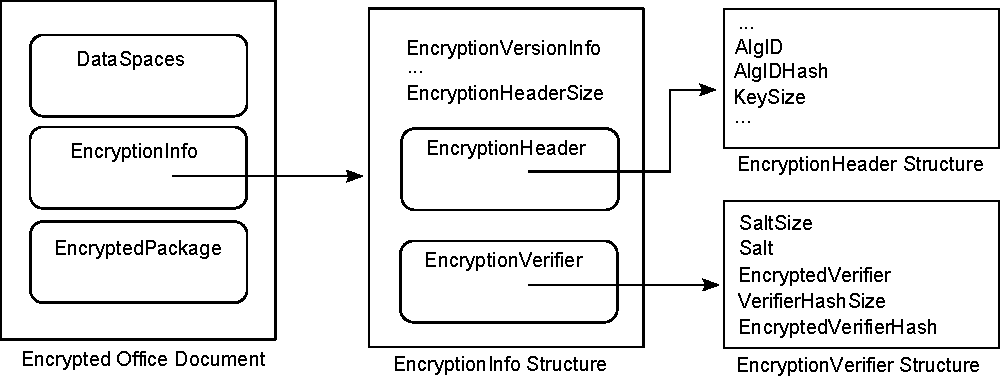
\includegraphics[width=1\textwidth]{figures/ei_struct.pdf}
	\caption{EncryptionInfo structure}
	\label{keys_length}
\end{figure}

Standard encryption describes three algorithms:
\begin{itemize}
	\setlength\itemsep{0.1em}
	\item{key derivation process,}
	\item{verifier generation process and}
	\item{password verification process.}
\end{itemize}

The key derivation process is derived from PKCS \#5: Password-Based Cryptography Version 2.0 as specified in RFC 2898 \cite{rfc2898} and the hashing algorithm used, specified in the \textit{EncryptionHeader.AlgIDHash} field, must be SHA-1. The exact steps to derive the encryption key are as follows:

\begin{enumerate}
\item{Calculate an initial password hash:}
	\begin{itemize}
		\item{$H_0 =\textit{SHA-1(salt + password)}$}
	\end{itemize}
\item{Iterate the hashing using the following approach: 
	\begin{itemize}
		\item{$H_n = \textit{SHA-1(iterator} + H_{n-1})$}
	\end{itemize}
	Variable \textit{iterator} is intially set to 0 and then incremented monotonically until 50,000 iterations have been performed.}
\item{Calculate a final hash:
	\begin{itemize}
		\item{$H_{final} = \textit{SHA-1}(H_n + block)$}
	\end{itemize}
	Variable $block$ is always $0x0000000$.}
\item{The final hash is XORed separately into the first 20-bytes of two buffers containing the bytes $0x36$ and $0x5C$ respectively. The two results of these operations are concatenated and the first $x$ bytes are considered to be the derived key, where $x$ is the key length required by the specified encryption algorithm.}
\end{enumerate}

The key is eventually used to encrypt the given document using AES in ECB mode. When attempting to decrypt the document in order to verify the correctness of a password entered, a password verifier is generated and stored within the \textit{EncryptionInfo} stream. The verifier is 16 bytes long and stored encrypted using AES in ECB mode and a key derived by the aforementioned method. In addition, an encrypted SHA-1 hash of the verifier is also stored. This information is used in the verification process as follows:

\begin{enumerate}
\setlength\itemsep{0.1em}
\item{Derive a key using the aforementioned method from the given user-password.}
\item{Decrypt the value stored in the \textit{EncryptedVerifier} field.}
\item{Decrypt the value stored in the\textit{EncryptedVerifierHash} field.}
\item{Calculate the SHA-1 hash value of the decrypted value calculated in step 2.}
\item{Compare the results of step 3 and step 4. 
	\begin{itemize}
		\item{In case the two values match the password is correct.}
	\end{itemize}}
\end{enumerate}

\begin{figure}[ht]
	\centering
	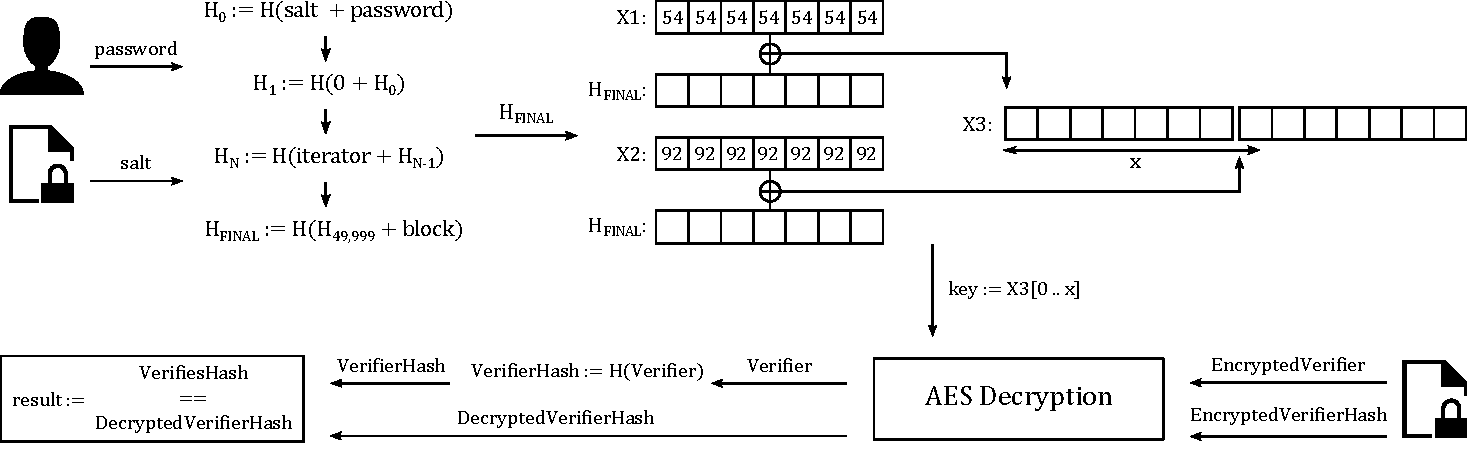
\includegraphics[width=1\textwidth]{figures/standard_encryption_scheme.pdf}
	\caption{Verification process as defined by ECMA-376 standard encryption}
	\label{standard_encryption_scheme}
\end{figure}

\subsection{Agile Encryption}

When agile encryption is used, all information about the cryptography used to encrypt the document is stored in an XML element in the \textit{XmlEncryptionDescriptor} field of the \textit{EncryptionInfo} stream. This element must conform to the XML schema namespace shown in \ref{ei_agilestream}. Agile encryption allows a wide range of possible configurations and is therefore much more complex than standard encryption discussed in the previous section. The available algorithms depend on the algorithms that can be accessed through the APIs in the Windows operating system. Microsoft Office 2007 with Service Pack 2 and above support CNG (CryptoAPI: Next Generation). The following listing shows the settings and their default values, which are configurable and change the way files are being encrypted:

\begin{itemize}
\setlength\itemsep{0.1em}
	\item{Set CNG cipher algorithm (default: AES).}
	\item{Configure CNG cipher chaining mode (default: CBC).}
	\item{Set CNG cipher key length (default: 128 bits).}
	\item{Specify encryption compatibility (default: Use next generation format).}
	\item{Set parameters for CNG context (see MSDN \cite{cng_functions}).}	
	\item{Specify CNG hash algorithm (default: SHA1).}
	\item{Set CNG password spin count (default: 100,000).}
	\item{Specify CNG random number generator algorithm (default: RNG).}
	\item{Specify CNG salt length (default: 16 bytes).}
\end{itemize}

A more detailed description of these settings can be found on the Microsoft Developer Network website\footnote{The settings and default values apply to Microsoft Office 2010 and 2013 and are identical.} \cite{plan_office_crypto}. 

Further specified are the steps necessary for deriving keys, generating initialization vectors, and generating a password key encryption structure. This structure is used to verify the correctness of the entered password when trying to open a file and it holds, encrypted, the key used to encrypt the plain-text document. Later in this chapter, this key is referred to as the intermediate key. Appendix \ref{ei_agilestream} shows the schema specifying its structure.

For the sake of completeness, it is important to mention that this structure can be represented as a \textit{CertificateKeyEncryptor} structure. The notable difference is that the intermediate key is encrypted using the public part of an X509 certificate instead of a user-supplied password. However, during the research no encrypted document was using this type of key encryptor structure nor was any information found about how to create a document using this type of protection. As a result this approach is not taken into account.

The key derivation process is similar to the method used in standard encryption and also derived from PKCS \#5 \cite{rfc2898}:

\begin{enumerate}
\item{Calculate an initial password hash:}
	\begin{itemize}
		\item{$H_0 =\textit{H(salt + password)}$}
	\end{itemize}
\item{Iterate the hashing using the following approach:}
	\begin{itemize}
		\item{$H_n = \textit{H(iterator} + H_{n-1})$}
	\end{itemize}
\item{Calculate a final hash:}
	\begin{itemize}
		\item{$H_{final} = \textit{H}(H_n + blockKey)$}
	\end{itemize}
\item{If the length of $H_{final}$ is smaller than the key length specified in the \textit{EncryptionInfo}, then the key must be padded by appending bytes with a value of $0x36$. If it is longer, it is truncated to the correct length.}
\end{enumerate}

Note that, unlike in standard encryption, $H()$ is not a fixed hashing algorithm and the $block$ variable depends on the purpose of the key that is being derived. Another difference is that $H_{final}$ is the final key.

Initialization vectors are generated as shown in the following steps:
\begin{enumerate}
	\item{If a \textit{blockKey} is provided the IV is:}
	\begin{itemize}
		\item{$H(KeySalt + blockKey)$}
	\end{itemize}
	\item{If a \textit{blockKey} is not provided, then the IV is the \textit{KeySalt}.}
	\item{Depending on the length, the IV is either padded by appending bytes with the value of $0x36$ or truncated to \textit{blockSize} (corresponding to the encryption algorithm specified) bytes.}
\end{enumerate}

\textit{KeySalt} is specified in the document's \textit{EncryptionInfo} and again, the \textit{blockKey} is determined by the IV's purpose.

To understand how the password key encryptor is generated, it is necessary to describe the meaning of some of its elements:

\begin{itemize}
\setlength\itemsep{0.1em}
	\item{\textbf{encryptedVerifierHashInput} -- a random array of bytes encrypted using a key derived using the user-supplied password and a fixed \textit{blockKey}: $0xfe, 0xa7, 0xd2, 0x76, 0x3b, 0x4b, 0x9e, 0x79$.} 
	\item{\textbf{encryptedVerifierHashValue} -- a hash of the plain-bytes of \textit{encryptedVerifierHashInput} encrypted using a key derived using the user-supplied password and a fixed \textit{blockKey}: $0xd7, 0xaa, 0x0f, 0x6d,$ $0x30, 0x61, 0x34, 0x4e$.}
	\item{\textbf{encryptedKeyValue} -- a random array of bytes encrypted using a key derived using the user-supplied password and a fixed \textit{blockKey}: $0x14, 0x6e, 0x0b, 0xe7, 0xab, 0xac, 0xd0, 0xd6$. This element represents the intermediate key.}
\end{itemize}

In addition to confidentiality, agile encryption also provides structures that are used to verify the integrity of encrypted files. These structures are stored in the \textit{EncryptionInfo's DataIntegrity} element. The process of generating this element is further described in \ref{data_integrity}. 

As a deduction from the aforementioned steps a randomly generated key is used to encrypt the plain-text content of the documents. Unlike in standard encryption where the final encryption key was directly derived from the user-supplied password. The specification does not mention anything about how this intermediate key should be generated. In case the key is not generated using a cryptographically secure pseudo-random number generator (CSPRNG), then an implementation specific weakness is introduced and presents a serious flaw in the encryption process. 

\subsection{Extensible Encryption} 

ECMA-376 documents can optionally utilize user-provided custom encryption modules. As this method is not commonly used it is not further analyzed or discussed.  

\section{Write Protection}

MS Office documents can be protected from unwanted changes. A user is allowed to open and read such files without restrictions. However, any kind of changes is prohibited. A password is required to authenticate the user and disable write protection. The Office Document Cryptography Structure mentions two different protection methods:

\begin{itemize}
\setlength\itemsep{0.1em}
	\item{ECMA-376 Document Write Protection and}
	\item{Binary Document Write Protection.}
\end{itemize}

In general, write protection is not meant to be a security mechanism \cite[p. 94]{msoffcrypto}. The protection can be easily bypassed, no matter which method was used. For this reason only a brief overview of the methods follows.

Write protection for documents represented in a binary format differs by document type:

\begin{itemize}
\setlength\itemsep{0.1em}
	\item{Word and PowerPoint documents -- the password is stored within the document file in plaintext\footnote{PowerPoint documents generated by MS Office PowerPoint 97-2007 Service Pack 1 will encrypt the whole file using the password \textit{/01Hannes Ruescher/01}. Starting with MS Office 2007 SP2 a binary write-protected PPT file will not be encrypted.}. The presence of the password indicates that the client application should enforce write protection.}
	\item{Excel documents -- the password is obfuscated before storing. The document can be encrypted when generated by MS Office Excel 2007 or above. However, this encryption is flawed as a well-known key: \textit{VelvetSweatshop}, is used. This is because the document should be readable for everyone. It helps to prevent direct modifications, i.e. by using a hex editor.}
\end{itemize}

Documents represented in a binary format that are intended to be compatible with ISO/IEC 29500 (Office Open XML File Format) and document files represented as specified in ECMA-376 store the password inside the document file in a hashed form. As an example MS Office Word 2013 will by default calculate the password hash as follows:

\begin{enumerate}
\item{Calculate an initial password hash:}
	\begin{itemize}
		\item{$H_0 =\textit{SHA1(salt + password)}$}
	\end{itemize}
	The salt is generated using an arbitrary pseudorandom function.
\item{Iterate the hashing 100,000 times using the following approach:}
	\begin{itemize}
		\item{$H_n = \textit{SHA1(iterator}+ H_{n-1})$}
	\end{itemize}
	Iterator is represented as a 32-bit integer initially set to 0.
\item{$H_{99,999}$ becomes the resulting hash.}
\end{enumerate}

Note that the iteration count and hashing function are configurable. This approach helps to protect the user-specified password when the document itself gets leaked to unathorized users. However, removing the whole hash entry from the file will effectively remove the write protection.

\section{Digital Signatures}\label{data_integrity}

\section{Summary}

\chapter{Portable Document Format}

Document protections of the Portable Document Format (PDF) files will be discussed in details necessary in context of this thesis. All information is based on two publicly available specifications:

\begin{itemize}
\setlength\itemsep{0.1em}
\item{Adobe® Supplement to the ISO 32000 \cite{iso32000sup} and}
\item{Document management — Portable document format — Part 1: PDF 1.7 \cite{pdf_spec}.}
\end{itemize}

The focus is on differences between various versions and how the protections evolved over time. As the file structure of PDF files is rather complicated and extensive the focus is, for the sake of simplicity, on parts specifically relevant to protection mechanisms.

\section{Encryption}

The encryption mechanism was introduced in PDF version 1.1. All encryption related information is stored in the document's trailer dictionary \cite[p. 42]{pdf_spec} within an encryption dictionary. The presence of the encryption dictionary implies that the document is encrypted.

Every encryption dictionary is required to specify the name of the preferred security handler for the document. The handler is a software module that implements aspects of the encryption process and controls access to the contents of an encrypted document. A standard password-based security handler is defined directly by the PDF specification. All algorithms discussed further in this chapter are specific for this standard security handler. It is important to note that while working on this thesis various tools where used to create PDF files and all these files implemented only the standard handler.

\subsection{Standard Security Handler}\label{pdf_enc}

Unlike other formats discussed (MS Office, Open Document Format) PDF's standard security handler allows the user to define access permissions and two passwords: an owner password and a user password. The user password is enough to decrypt a document. The owner password is needed in case the user wants to modify the access permissions of the document.

Table \ref{handler_entries} shows encryption dictionary entries defined by the standard security handler which are important in the algorithms described later in this chapter.

\begin{table}[hp]
	\centering
	\begin{tabular}{|l|l|}
               	\hline
		\textbf{Key}&\textbf{Value}\\
		\hline
		V&Specifies the algorithm used to encrypt \\
		&and decrypt the document.\\
		&\textbf{0} -- An algorithm that is undocumented.\\
	`	&This value shall not be used.\\
		&\textbf{1} -- RC4 or AES with a key of length 40 bits.\\
		&\textbf{2} -- RC4 or AES permitting keys longer then 40 bits.\\
		&Available since PDF 1.4.\\
		&\textbf{3} -- An unpublished algorithm permitting keys\\
		&of lengths from 40 to 128 bits.\\
		&This value shall not be used in conforming PDF files.\\
		&\textbf{4} -- A more sophisticated encryption and decryption\\
		&process using rules defined in additional entries\\
		&of the dictionary. Available since PDF 1.5.\\
		&\textbf{5} -- Same as 4 but allows the use of keys with length\\
		&256 bits.\\
	\hline
		R&Specifies the revision of the security handler.\\
		&Can have values from 2 to 5 and mostly depends on V.\\
	\hline
		O&A 32-byte (for R being 1-4) or 48-byte (for R being 5)\\ 
		&string based on both the owner and the user password.\\
		&Used in the owner password verification process.\\
	\hline
		U&A 32-byte (for R being 1-4) or 48-byte (for R being 5)\\ 
		&string based on the user password.\\
		&Used in the user or owner password verification process.\\
	\hline
		P&A set of flags representing access permissions.\\
	\hline
		EncryptMetadata& In case V is of value 4 (PDF 1.5) indicates\\
		&if document metadata should be encrypted.\\
	\hline
           \end{tabular}
	\caption{Encryption dictionary entries defined by the standard security handler \cite{pdf_spec}}
	\label{handler_entries}
\end{table}

The owner-based or user-based encryption keys are computed using the following algorithm by standard security handlers of revision 1-4: 

\begin{enumerate}
\setlength\itemsep{0.1em}
\item{If the password is longer than 32 bytes\footnote{The password is represented in PDFDocEncoding \cite[157]{pdf_spec}. 32 bytes can represent 32 characters.} use only its first 32 bytes. Otherwise, pad it by appending bytes from the beginning of the following default 32-byte padding string: $28$ $BF$ $4E$ $5E$ $4E$ $75$ $8A$ $41$ $64$ $00$ $4E$ $56$ $FF$ $FA$ $01$ $08$ $2E$ $2E$ $00$ $B6$ $D0$ $68$ $3E$ $80$ $2F$ $0C$ $A9$ $FE$ $64$ $53$ $69$ $7A$. In case no user-password is provided, the whole padding string is used.}
\item{Using a MD5 hash function compute a hash of the following data:}
	\begin{itemize}
		\item{The result of step 1.}
		\item{The encryption dictionary's O entry.}
		\item{The encryption dictionary's P entry.}
		\item{The first element of the file's identifier array \cite[p. 43]{pdf_spec}.}
		\item{4 bytes with the value $0xFFFFFFFF$ if document metadata is not being encrypted.}
	\end{itemize}
\item{For revision 3 or greater hash the first $n$ bytes of the output using MD5, where $n$ is the length of the required encryption key as defined in the encryption dictionary. Repeat this step 50 times.}
\item{The first $n$ bytes become the computed encryption key.}
\end{enumerate}

The O entry is basically the user password encrypted by a owner-password-based key. The algorithm is as follows:

\begin{enumerate}
\setlength\itemsep{0.1em}
\item{Pad or truncate the owner password the same way as described in the previous algorithm.}
\item{Hash the output of step 1 using the MD5 hash function.}
\item{For revision 3 or greater hash the output of previous step using the MD5 hash function. Repeat this step 50 times.}
\item{Use the first $n$ bytes as an RC4 encryption key, where $n$ is 5 for handlers of revision 2. For handlers of revision 3 or greater $n$ is the length of the encryption key as defined in the encryption dictionary.}
\item{Pad or truncate the user password the same way as described in the previous algorithm and encrypt it using RC4 with the key obtained in the previous step.}
\item{For revision 3 or greater repeat the following 19 times: Take the output of the previous invocation of RC4 and pass it as input to a new invocation. The encryption key for every iteration is created by performing an XOR operation between each byte of the encryption key obtained in step 4 and the byte value of the iteration counter (values 1-19).}
\end{enumerate}

The U entry is for handlers of revision 2 the default 32-byte padding string encrypted using the user-password-based encryption key. For handlers of revision greater than 3 the way how the U entry is calculated changed. The algorithm is as follows:

\begin{enumerate}
\setlength\itemsep{0.1em}
\item{Using a MD5 hash function compute a hash of the following data:}
\begin{itemize}
		\item{the default 32-byte padding string, and}
		\item{the first element of the file's identifier array \cite[p. 43]{pdf_spec}.}
\end{itemize}
\item{Encrypt the result using RC4 with the user-password-based encryption key.}
\item{Do the following 19 times: Take the output of the previous invocation of RC4 and pass it as input to a new invocation. The encryption key for each iteration is created by performing an XOR operation between each byte of the encryption key obtained in step 4 and the byte value of the iteration counter (values 1-19).}
\item{Append 16 bytes of arbitrary padding to the output of the previous step.}
\end{enumerate}

Note that the user-password-based encryption key is used to decrypt contents of the document. The owner-password-based key is used to verify correctness of the provided owner-password.

In revision 5 all algorithms previously mentioned were completely replaced. Two new encryption dictionary entries were introduced (see table \ref{additional_handler_entries}). 

\begin{table}[h]
	\centering
	\begin{tabular}{|l|l|}
               \hline
		\textbf{Key}&\textbf{Value}\\
	\hline
		OE&A 32-byte string based on the owner and user passwords.\\
		UE&A 32-byte string based on the user password\\
	\hline
           \end{tabular}
	\caption{Encryption dictionary entries introduced by standard security handlers of revision 5}
	\label{additional_handler_entries}
\end{table}

The maximum password length was extended from 32 bytes to 127 bytes. As mentioned before the U and O entries were extended to 48 bytes and represent 3 logical parts. The first 32 bytes are a verification hash. The next 8 bytes are a validation salt. The last 8 bytes are a key salt. The OE and UE values contain the file encryption key encrypted by the an owner-password-based or user-password-based key respectively.

At this point the publicly available supplement to the ISO 32000 \cite{iso32000sup} appears to be incomplete in terms of the file's encryption key computation. A new "Computing an encryption key" algorithm is described. This algorithm includes a step where decrypting the OE, or UE, value is necessary to get the file encryption key. Algorithms to generate the OE and UE values include a step where encrypting the file encryption key is necessary. However, the origin of the file encryption key is not mentioned. 

The process of password verification is straightforward:

\begin{enumerate}
\setlength\itemsep{0.1em}
\item{Truncate the provided password to 127 bytes\footnote{The password is based on Unicode (UTF-8 encoding).} if it is longer than 127 bytes.}
\item{Compute the SHA-256 hash of the password concatenated with 8 bytes of the owner validation salt and the 48-byte U value.}
\item{In case the result matches the 32-byte verification hash of the O value, the provided password is the correct owner password.}
\item{Compute the SHA-256 hash of the password concatenated with 8 bytes of the user validation salt.}
\item{In case the result matches the 32-byte verification hash of the U value, the provided password is the correct user password.}
\end{enumerate}

An interesting observation can be seen after describing the way of verifying a password provided by the user. The only computation that has to be done to verify a given password is calculating one SHA-256 hash value. This approach actually weakens the strength of the document protection as discussed in more detail in section \ref{pdf_summ}.

\section{Watermark Annotations}

\section{Signature Fields}

\section{Summary}\label{pdf_summ}

\chapter{Open Document Format for Office Applications}

Documents in the Open Document Format can be represented in two ways \cite{odt_spec}:

\begin{itemize}
\setlength\itemsep{0.1em}
\item{A single XML document.}
\item{A collection of files within a package, each of which stores a part of the document.}
\end{itemize}

Particularly important in context of this paper is the latter way mentioned. All protection mechanisms defined apply to packages. A package representing a single Open Document Format file will be referred to as “ODT package” from now on.

\section{Encryption}\label{odt_enc}

The encryption process as specified in Open Document Format for Office Applications (\textit{OpenDocument}) \cite{odt_spec} has 3 stages:

\begin{enumerate}
\setlength\itemsep{0.1em}
	\item{The user-supplied password is hashed.}
	\item{For each file to be encrypted a separate key is generated using the hashed password and the PBKDF2 algorithm \cite{rfc2898}.}
	\item{The files are encrypted using the keys created in step 2.}
\end{enumerate}

The exact algorithms and other necessary cryptographic parameters are defined in the document's manifest. The manifest is a mandatory part of every ODT package and its relative path within the package must be \texttt{META-INF/}
\texttt{manifest.xml}. The manifest is an XML file conforming the XML schema shown in Appendix B.

For every file in the ODT package the manifest must contain an element denoted as \texttt{<manifest:file-entry>}.

\begin{figure}[ht]
	\centering
	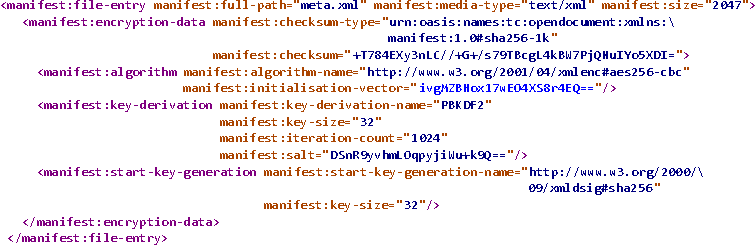
\includegraphics[width=1\textwidth]{figures/manifest_snippet.pdf}
	\caption{Example of a file entry element within an ODT document's manifest file}
	\label{manifest_snippet}
\end{figure}

A \texttt{<manifest:encryption-data>} child element indicates that the file is stored encrypted within the package. It also contains information required to decrypt the particular file. The attribute \texttt{manifest:checksum-type} specifies a digest algorithm used to calculate a hash of the file. This hash is stored in the \texttt{manifest:checksum} attribute in BASE64 encoding. 
The algorithm used to encrypt a file is specified in the \texttt{manifest:algorithm-name} attribute of the \texttt{<manifest:algorithm>} element. In case this algorithm requires an initialization vector it is specified in the \texttt{manifest:initialization-vector} attribute.
In a similar fashion the elements \texttt{<manifest:key-derivation>} and \texttt{<manifest:start-key generation>} specify how the start key is generated from the user password and how the encryption key is derived from the start key, respectively.
All algorithms that can be used for the purposes discussed in this section and should be supported by implementations are listed in the Open Document Format specification. New algorithms were added as the specification was extended over time. 

Versions 1.0 and 1.1 specified SHA-1 as the only hash function for the \texttt{manifest:checksum-type} and \texttt{manifest:start-key-generation-name} attributes. The only available \texttt{manifest:algorithm-name} was Blowfish in CFB mode. Version 1.2 introduced support for additional hash functions and algorithms: SHA-256, SHA-512, RIPEMD-160, 3DES, AES-128, AES-256 and AES-192. The only available key generation algorithm in all three versions is PBKDF2.

\section{Digital Signatures}

Digital signatures are defined beginning with version 1.2. One package may contain more signatures. The signatures are located within the \texttt{META-INF/} folder and should contain the term "signature" in their name. Every signature has to explicitly list all files which are being validated. In particular to ensure integrity of the whole document, all files should be referenced by some signature. 

The Open Document Format specification describes that digital signature can be used together with encrypted packages in two ways. The signature can be applied on encrypted files and should be validated prior to decrypting the package. The other option is digitally signing the package before encrypting it. This approach will also encrypt the files containing digital signatures.  

However, popular implementations seem to only support the first mentioned approach. Once a digitally signed file is encrypted, they will remove all signatures before encrypting the file. The file has to be manually resigned again. 

\section{Summary}

Protections described in the Open Document Format are rather simple and unambiguous. Focus on security can be seen looking at differences of various versions. Version 1.2 introduced a mechanism for digital signatures as well as support for modern cryptographic functions. The use of PBKDF2 with configurable iteration count allows mitigating simple offline brute-force attacks. However, GPU powered attacks may become extremely successful as PBKDF2 is not designed to be memory-hard \cite{PBKDF2_attack}.

Two popular implementations have been tested: LibreOffice \cite{libreoffice} and Apache OpenOffice \cite{openoffice}. Both application were used in the latest available stable version at the time. For Libre Office this was version 5.2.2 and for Open Office version 4.1.3. On overview of the results is shown in table \ref{odt_impl_results}.

\begin{table}[h]
	\centering
	\begin{tabular}{|l|l|l|}
               \hline
		&\textbf{LibreOffice}&\textbf{Apache OpenOffice}\\
	\hline
		manifest:checksum-type&SHA-256&SHA-1\\
	\hline
		manifest:algorithm-name&AES-256&Blowfish CFB\\
	\hline
		manifest:start-key-derivation-name&SHA-256&SHA-1\\
		manifest:key-derivation-name&PBKDF2&PBKDF2\\
		manifest:iteration-count&1024&1024\\
		manifest:key-size&32&16\\
	\hline
           \end{tabular}
	\caption{Comparsion of document protections methods used by LibreOffice and Apache OpenOffice}
	\label{odt_impl_results}
\end{table}

Both applications encrypt all files in the package. Similarly both applications include all files when applying a digital signature to the document. A particular interesting finding is that Open Office prefers the Blowfish algorithm to encrypt documents.

\chapter{Distributed Password Recovery}

As people tend to forget passwords, it is likely, that access to password protected documents can be lost. A straight-forward solution in this case is brute-force, as password verification is done offline. To show and further discuss the speed and efficiency of this process a distributed password recovery system was created.

The whole implementation and any files mentioned in this chapter can be found on the attached CD or in the official thesis archive available at \textit{http://is.muni.cz/}.

\section{System Overview}

The whole system consists of 3 logically separated parts depicted in figure \ref{ddpbf_design}. 

\begin{figure}[ht]
	\centering
	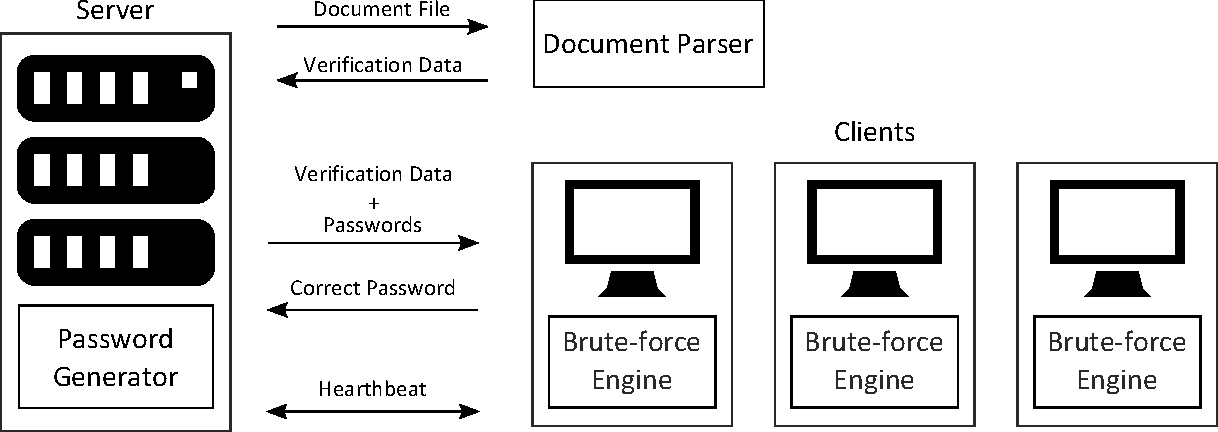
\includegraphics[width=1\textwidth]{figures/ddpbf_design.pdf}
	\caption{Distributed password recovery design}
	\label{ddpbf_design}
\end{figure}

The input for the system is a password protected Office, PDF or ODT document. As the password verification process can be very different among these formats, a detailed list of currently supported algorithms follows:

\begin{itemize}
\setlength\itemsep{0.1em}
	\item{MS Office Document Structure -- Standard Encryption (as described in subsection \ref{msoff_standard_enc}).}
	\item{Portable Document Format --  version 1.3 to 1.7 using standard security handlers from version 1 to 5 and revision 2 to 6 (as described in subsection \ref{pdf_enc}).}
	\item{Open Document Format – version 1.2 using AES-256 (as described in subsection \ref{odt_enc}).}
\end{itemize}

The basic idea is that the server part serves as the main entry point for the user and handles all additional work. It utilizes a document parser to gather information necessary for password verification and distributes work among all active clients. A more detailed description of every part follows. 

\subsection{Client-server model}\label{client-server}

The server provides a simple command line interface and can be started using the following command: 

\begin{lstlisting}
$ python server.py [-h] [-pr PASSWORDRANGE] [-ps PAYLOADSIZE] document_type filename tcp_ip tcp_port
\end{lstlisting}

Note that the current version must be run with Python 2.7 in order to function properly. A detailed description of the arguments follows:

\begin{itemize}
\setlength\itemsep{0.1em}
	\item{\textbf{-h} -- Shows a descriptive help message.}
	\item{\textbf{-pr} -- Sets the password's maximum length (default: 8).}
		\begin{itemize}
		\setlength\itemsep{0.1em}
			\item{All passwords up to the specified length will be checked.}
		\end{itemize}
	\item{\textbf{-ps} -- Number of passwords sent to each client on every connection (default: 20,000).}
	\item{\textbf{document\_type} -- Number identifying the given document's type.}
		\begin{itemize}
		\setlength\itemsep{0.1em}
			\item{1 -- Microsoft Office}
			\item{2 -- Open Document Format}
			\item{3 -- Portable Document Format}
		\end{itemize}
	\item{\textbf{filename} -- Path to the document file which's password should be recovered.}
	\item{\textbf{tcp\_ip, tcp\_port} --  IP address and port number to which clients should connect in order to communicate with the server.}
\end{itemize}\label{server_params}

When run, the server extracts all information necessary to perform the password recovery process. This is accomplished by calling one of the document parsers described in subsection \ref{doc_parsers}. Afterwards the server is passively waiting for clients to connect. Once connected the server sends the verification data and a list of passwords in JSON \cite{rfc7159} format:

\begin{lstlisting} 
{"passwords":[<passwords>], "data":"<document_parser_output>"}
\end{lstlisting}\label{server_message}

Passwords are generated in a separate sub-process and placed into a synchronized queue. To prevent massive memory consumption the number of items in the queue must never exceed the limit of 2 times the password chunk size that is sent to clients (set by the \textit{–pr} argument).

A list of active clients is maintained by the server. Every client is clearly identified by a universally unique identifier (UUID) \cite{rfc4122}. When setting the \textit{–pr} argument to a high value the time interval between two messages exchanged between a client and the server might be very high (even days). This is because, the client will ask for a new list of passwords after it successfully verifies all the passwords it received. To recognize inactive clients (e.g. the client machine was terminated etc.) a hearth beat mechanism is implemented. Every 20 seconds a small message (hearth beat) is sent to the server. As a result, any client not connecting to the server for longer than 120 second will be marked as inactive. In case the client connects at any later point, it will be treated as a new client. There is no maximum number of clients, which allows theoretically an unlimited linear growth in performance. The server keeps track of what passwords were sent to which client. This prevents losing passwords in case a client becomes unresponsive. Once a client is marked inactive all passwords that were currently processed by it are eventually resend to another client. 

On every client connection (excluding heart beats) an update is logged. This update contains the current number of active clients and an estimate of the current recovery speed. Every password has to go through a hashing process to be verified. Therefore, the speed is represented by the number of tried passwords per second. The speed is naively computed as the ratio of the elapsed time and passwords processed by clients. This implies that the server cannot estimate a speed before at least one client asks repeatedly for more passwords. The server will automatically shutdown in case it receives the correct password from a client.

The client can be run using the following command:
\begin{lstlisting}
$ python client.py [-h] tcp_ip tcp_port 
\end{lstlisting}

The \textit{tcp\_ip} and \textit{tcp\_port} are the connection parameters used to communicate with the server. The optional \textit{–h} argument will show a descriptive help message. 

Once run, the client generates a UUID and immediately sends a message to the server asking for a password list and the verification data. This information is then passed to the brute-force engine described in subsection \ref{brute_force_engine}. The actual brute-forcing is separated from the client on purpose. The reason for this is to keep the system as modular as possible. It is important to note that this approach allows any brute-force engine to be used (e.g. hashcat or JtR \cite{hashcat, jtr} described in more detail in section \ref{related_work}). When done the result is sent to the server. In case the password was not found, the client will receive a new password list and repeat the whole process.

\subsection{Document parsers} \label{doc_parsers}

The document parsers are stand-alone Python scripts that take document files as input and return all  data necessary for the verification process. Note that the scripts used to extract information from PDF and MS Office files were not created as part of this thesis, but rather taken from the public \textit{John the Ripper} GitHub repository.\footnote{Available at \textit{https://github.com/magnumripper/JohnTheRipper}} Small modifications were made to these scripts, to better fit into the developed system. All changes are included as comments in the respective files. Parsing of ODT files was implemented as part of this thesis. The parser accepts as valid input ODT files conforming the latest specification (version 1.2).

\subsection{Brute-force engine}\label{brute_force_engine}

The brute-force engine can be used either as a stand-alone Python script providing a simple command line interface, or as a Python module. When run separately it can be started using the following command:

\begin{lstlisting}
$ python brute_force.py [-h] [-pr PASSWORDRANGE] document_type filename
\end{lstlisting}

All the parameters correspond to the identically named parameters described in subsection \ref{server_params}. Once the engine is invoked this way, it parses the given document and initializes a password range based brute-force process. Passwords are generated and placed in a synchronized queue in a separate process. The passwords in the queue are being pulled one by one and verified using a \textit{password verifier}. There are 3 separate verifiers for the supported documents respectively. All three verifiers are written in plain C and the script utilizes Python's multiprocessing module to invoke more instances simultaneously. C was chosen for performance reasons, as it was shown that a plain rewrite from Python to C speeded up the verification process by approximately 4 times. The code snippet below shows the methods responsible for calling these verifiers.

\begin{lstlisting}
def _call_msoffcrypto_core(pwd, input_data):
    return Popen(["ms-offcrypto-impl/./msoffcrypto", pwd, 
        input_data[5], # salt
        input_data[4], # salt_length
        input_data[6], # encrypted_verifier
        str(len(input_data[6]) / 2), # enc_verifier_length
        input_data[7], # encrypted_verifier_hash
        str(len(input_data[7]) / 2), # enc_verifier_hash_length
        str(input_data[3]), # aes_key_length
        str(input_data[2]), # verifier_hash_size
        ])

def _call_odt_core(pwd, input_data):
    return Popen(["odt-impl/./odt", pwd, 
        input_data[2], # checksum
        input_data[3], # iv
        input_data[4], # salt
        input_data[5], # encrypted_file
        str(input_data[6]), # encrypted_file_length
        ]) 

def _call_pdf_core(pwd, input_data):
    return Popen(["pdf-impl/./pdf", pwd, 
        input_data[1], # version
        input_data[2], # revision
        input_data[3], # length
        input_data[4], # p
        input_data[5], # meta_encrypted 
        input_data[6], # id_length 
        str(input_data[7]), # id
        input_data[8], # u_length 
        str(input_data[9]), # u 
        input_data[10], # o_length
        str(input_data[11]) # o
        ]) 
\end{lstlisting}


In a similar fashion these verifiers can be called directly and accept a \textit{–v} argument to enable verbose output for debugging purposes. Note that the verifiers use the OpenSSL library for C \cite{openssl} to perform all cryptographic operations. Therefore, when compiling them it is necessary to add a link to the library (i.e. using \textit{-lssl} and \textit{-lcrypto} switches when compiling with \textit{GCC}).

Additionally the script provides a public \textit{init()} method, which requires either a password range or a list of passwords as an argument. If a password range is given the script generates its own list. This is done using a naive generator which generates all possible variations of words consisting of lower case letters up to the given range. As an example, if the specified range is 2 then the resulting generated word list contains the characters 'a' to 'z' and words 'aa' to 'zz'. Otherwise the provided list of passwords is directly placed in a synchronized processing queue. The second approach is used in the client-server model discussed in subsection \ref{client-server}. It is important to note that this allows the engine to be easily modified to use a wordlist as input. A wordlist approach can in general be more efficient then plain brute-forcing of passwords, resulting in a faster password recovery.

\section{Related Work}\label{related_work}

\section{Testing and Results}

\chapter{Conclusion}

\begin{thebibliography}{}
	\bibitem{msoffcrypto}Microsoft Corporation. 2015 \textit{[MS-OFFCRYPTO]: Office Document Cryptography Structure.} [ONLINE].
Available at: \\ \textit{https://msdn.microsoft.com/en-us/library/office/cc313071(v=office.12).aspx.} [Accessed 18 September 2016]
	\bibitem{rfc2898} B. Kaliski. 2000 \textit{PKCS \#5: Password-Based Cryptography Specification Version 2.0.} [ONLINE].\\ Available at: \textit{http://www.ietf.org/rfc/rfc5246.txt} [Accessed 18 September 2016]
	\bibitem{cng_functions}Microsoft Corporation. 2016 \textit{CNG Cryptographic Configuration Functions.} [ONLINE].
Available at: \\ \textit{https://msdn.microsoft.com/en-us/library/bb204774(v=VS.85).aspx.} [Accessed 18 September 2016]
	\bibitem{plan_office_crypto}Microsoft Corporation. 2014 \textit{Plan cryptography and encryption settings for Office 2013.} [ONLINE].
Available at: \\ \textit{https://technet.microsoft.com/en-us/library/cc179125.aspx.} [Accessed 18 September 2016]
	\bibitem{odt_spec}OASIS Standard. 2011 \textit{Open Document Format for Office Applications (OpenDocument) Version 1.2.} [ONLINE]. Available at: \textit{http://docs.oasis-open.org/office/v1.2/OpenDocument-v1.2.html.} [Accessed 19 September 2016]
	\bibitem{rfc7159} T. Bray, Ed. 2014 \textit{The JavaScript Object Notation (JSON) Data Interchange Format} [ONLINE].\\ Available at: 	\textit{https://tools.ietf.org/rfc/rfc7159.txt} [Accessed 30 October 2016]
	\bibitem{rfc4122} P. Leach, Microsoft, M. Mealling, Refactored Networks, LLC, R. Salz, DataPower Technology, Inc.  2005 \textit{The JavaScript Object Notation (JSON) Data Interchange Format} [ONLINE].\\ Available at: \textit{https://tools.ietf.org/rfc/rfc4122.txt} [Accessed 30 October 2016]
	\bibitem{hashcat}\textit{hashcat - advanced password recovery.} [ONLINE].
Available at: \\ \textit{https://hashcat.net/hashcat/.} [Accessed 30 October 2016]
	\bibitem{jtr}\textit{John the Ripper password cracker.} [ONLINE].
Available at: \\ \textit{http://www.openwall.com/john/.} [Accessed 30 October 2016]
	\bibitem{openssl}OpenSSL Software Foundation. 2016 \textit{Welcome to OpenSSL!.} [ONLINE].
Available at: \\ \textit{https://www.openssl.org/.} [Accessed 30 October 2016]
\end{thebibliography}





\begin{appendix}
	\chapter{Attachements}
	\section{[MS-OFFCRYPTO] Structures and Schemas}\label{msoffcrypto_structs}
	\subparagraph{EncryptionInfo Stream (Standard Encryption)}\label{ei_standardstream}

	\subparagraph{EncryptionInfo Stream (Agile Encryption)}\label{ei_agilestream}.
\end{appendix}
\end{document}

